\chapter{附录伽罗瓦与群论}
\begin{center}
	L . R . 利伯著 , 樊?译
\end{center}

\section{引言}

大家都知道:科学知识是与时俱进的 , 科学是一种活的 , 蓬勃 滋长的东西 . 然而一般人总把数学看做又老又朽 , 似乎再也不能 滋长发扬的了 . 的确 , 在学校里所教的数学——算术 , 代数 , 几何——在几世纪前大家早都知道;就是专门学院的教程差不多也有 三百多年的历史 . 笛卡儿(Descartes)之创造解析学和牛顿(Newton)之发明微积分 , 那都是十七世纪的事情 . 可是 , 事实是这样 的:数学的范围甚至比科学的范围还要来得广些 , 就从那个时候 起 , 他已在脚踏实地的向前迈进了 . 

数学中一些比较新颖的概念是什么?是不是他们太抽象了 ——虽然好些概念还是由很年轻的数学天才所创的——使得这一 代的青年人连听都够不上听一听呢?是不是他们距离平常的一般 思维方法太远了 , 以致不能使一般普通的人们从中得到任何用处 和快乐?难道连一般数学教员对于这些概念也不能有一个认识的 机会吗?不是的!其实是这样的:那些近代数学上的发展不但能 使数学家发生兴趣 , 而且正像微积分一样 , 对于科学家也能有相当 伟大的帮助 . 哲学家公认:近代数学与基本的宇宙观是有直接关 系的 . 心理学家在近代数学中也会看到一种能从偏见中把心胸解 放出来的以及能在陈腐的偏见之荒墟上建立起簇新有力之结构来 的伟大王具——像是在非欧几里得几何学之创造中所可以看到 的 . 的确 , 谁都要珍重现代数学之特殊的旺盛和卓绝的本色 . 

这本小册子 , 作者有心想把他当做现代数学中一支的入门 , 使 得那些对于这门数学愿作更进一步研究的人们在阅读时较为容易 些有趣些 . 

这本小册子里所讲的是群论(Theory of Groups) , 群论是近代数学的一种 . 

伽罗瓦(Évanste Galois)对于这门数学的理论和应用很多发扬 . 伽罗瓦殁于一百年以前\footnote{译者按:伽罗瓦卒于1832年 , 此书原本系在1932年出版 , 所以原书作者说: “伽罗瓦殁于一百年以前” . } , 死的时候还不满二十一岁 . 在他那短促而悲惨的生命中 , 于群论颇多贡献;而这门数学 在今日已成为数学中的重要部分了 . 自古以来的二十五位大数学家中 , 他就是其中之一位\footnote{G . A . Miller in Science , Jan . 22 , 1932 . } . 

他的一生 , 除了在数学上有惊人的成功 , 其余尽是失意的事 . 

他渴望着进巴黎的L'Ecole Polytechnique , 但在入学考试时竟失 败了;过了一年 , 他再去应试 , 然而仍旧是失败 . 他拿自己研究的 结果给歌西(Cauchy)和傅利(Fourier)二氏看 , 这两人是当时很出 色的数学家 , 但是他们对他都没有注意 , 而且两人都把他的稿本抛 弃了 . 他的师长们谈起他的时候 , 常说:“他什么也不懂” . 他没 有智慧 , 不然就是他把他的智慧隐藏得太好了 , 使我简直没法子去 发见他” . 他被学校开除了 . 又因为是革命党徒 , 曾经被拘入狱 .  他曾与人决斗 , 就在这决斗中他是被杀了 . \footnote{在决斗的前夜 , 他自己预知必死 . 仓猝中将自己在数学上的心得草率写出 , 交给他的一个朋友(参看Annales de L'Ecole Normale Supérieure ,  1896 中M . P .  Dupuy所作之伽罗瓦传 , 或参阅David Eugene Smith味著之Source Book in Mathematics 一书 . )}

敬祝他的灵魂安乐!

\section{群的重要}

在讲群论之先 , 先把群论之所以重要的几个原因之一说一下 . 

我们都知道数学中一桩要紧的事情是解方 程式 . 代数方程式\footnote{代数方程式是作
	\[
	a_{0} x^{n}+a_{1} x^{n-1}+\cdots \cdots+a_{n}=0
	\]
	的形式的方程式 , 此中 $n$ 是正整数 . }可以依他的次数来分类 . 一次方程式\footnote{$a=0$ 而 $b \neq 0$ 的情形除外 . }
\[
a x+b=0
\]
只要是学过初等代数的小孩子都会解\footnote{一次方程式的解法是在纪元前 1700 年发明的 ,  这年代是根 据 Ahmes Papyrus 书中的记载 . 此抄本是一部最早的数学文献 , 现已得美国数学会之贫助而出版 . } ,  他的解答是
\[
x=-\dfrac{b}{a} . 
\]
二次方程式
\[
a x^{2}+b x+c=0
\]
的解法在初等代数中也有 , 他的解答是
\[
x=\dfrac{-b \pm \sqrt{b^{2}-4 a c}}{2a}
\]
在纪元前数世纪 ,  巴比伦人(Babylonians)已能解这种形状的方程
式了\footnote{参阅 School and Society , June 18 , 1932 , p . 833 , G . A , Miller 著之 The Oldest Extant Mathematics 一文 . } . 

三次方程式
\[
a x^{3}+b x^{2}+c x^{2}+d=0
\]
和四次方程式
\[
a x^{4}+b x^{3}+c x^{2}+d x+e=0
\]
的解法已比解一次、二次的方程式难得多了 . 直到十六世纪才有了解法 . 这法子在每本方程式论的书中都可以找到 . 

当方程式的次数增大时 , 解法的田难增加得很快 . 向来数学家虽都不会解一般高于四次的方程式 , 可是都相信一定 是可能的\footnote{即如十八世纪的大数学家欧拉(Euler)也相信这是可能的} . 直到十九世纪 , 利用群论的道理 , 才证明了这 是 不可能的事 . 

此处读者应该要懂得透彻的是刚才所说的“不可能”三个字 . 一个问题之能否解决是要看我们对于解答所加的限制条件而定的 . 譬如
\[x+5=3\]
是能解的 , 假使我们允 许$x$可以是负数的话 . 设若我们限定$x$不能是 负数 , 那末 , 这方程式就 不能解了 . 

同样 , 假使$x$表示 银圆数 , 方程式
\[2x + 3=10\]
是可解的 . 如果$x$表示 人数 , 这方程式就不能 解了 , 因为$x=3\dfrac{1}{2}$没有 意义 . 

要三等分任意一 角 , 若只准用直尺与圆 规 , 这是不可能的 . 但是若许用别的仪器 , 就可能了 . 

一个代数式之为\emph{可约的}(reducible , 就是说可以分解因数)或\emph{不可约的}(irreducible) , 要看我们在什么\emph{数域}(Field)\footnote{一个数域是一个数的集合 , 其中任二数的和 , 差或积或商(但零不许作除数)仍 在这集合中 . 故所有复数做成一个数域;所有实数也做成一个数域;所有有理数也做 成一个数域 . 但是一切整数的集合不成一个数域 . 因为两个整数的商不一定还是整 数 . 许多有趣的数域的例子 , 可以在L . W . Reid之The Theory of Algebraic Numbers 书中看到 . }中分解因数而定 . 譬如
\[
x^{2}+1
\]
在\emph{实数域} (Field of Real Numbers) 中是不可约的 , 可是在\emph{复数域}(Field of Complex Numbers)中却是可约的 ,  因为
\[
x^{2}+1=(x+i)(x-i) , 
\]
此处的 $i=\sqrt{-1}$  . 简单的说: 我们若单说一个代数式是可约的 或是不可约的 , 而不说出在什么数 域内 , 这话是全然没有意义的 . 

数学家知道特别说明\emph{范围}(Environment)的重要 . 我们说:一 个命辞在什么范围中是对的 , 在什么范围中是错的 , 甚而至于在什 么范围中是绝对没有意义的 . 

那末 , 刚才所说一般高于四次的方程式不能解究竟是什么意思呢?这问题的答案是:一般高于四次的方程式是不能用根式解 的 . 所谓“不能用根式解”是说方程式的根不能用有限次的有理运 算(加、减、乘、除)和开方表作方程式的系数之函数 . 

为要说明这一点 , 拿一次方程式
\[ax+b = 0\]
来看 , 这方程式的根是
\[
x=-\dfrac{b}{a} . 
\]

所以 $x$ 的值可以用a除b而得 , 这是一个有理运算 三次方程式
\[
a x^{2}+b x+c=0
\]
的两个根是
\[
x=\dfrac{-b \pm \sqrt{b^{2}-4 a c}}{2a}
\]
这也可以由有限次的有理运算和开方而得 . 

同样 , 一般的三次、四次方程式的根也可用有限次的有理运算和开方表作系数的函数 . 换句话说:他们可以\emph{用根式解}(Solvable by Radicals) , 

可是 , 若论到高于四次的方程式时 , 这就不再成立了 . 当然 ,  这是指一般高于四次的方程式而言 , 有些特殊的高次方程式还是 可以用根式解的 . 

以后我们将看到怎样用群论的原理来证明一般高于四次的方 程式是不能用根式解的\footnote{(若不限定单用有理运算和开方来解高于四次的方程式 , 关于这点 , 可参读L .  E . Dickson的Modem Algebraic Theories以及该书中所指的参考书[这当然不是 指近似解法如图解法或霍纳氏法(Homer's method)等而言的 , 这类近似解法只在应 用数学上有用] . } . 

我们还可以看到:用群论的道理来证明以直尺、圆规三等分任 意角之不可能是何等简单而绮丽 , 正如应用群论于其他名题一样!

\section{群是什么}

数学中的系统(System)可以说是一部数学的机器(A Mathematical Machine) , 他的主要成分是

(1)元素(Element) . 

(2)	—种运算(Operation) . 

例如 , 

(a)(1)元素是一切整数(正或负或0);

(2)运算是加法 . 

(b)(1)元素是一切有理数\footnote{一个有理数是一个可以写做两个整数的商的数 . 譬如$3/5$是一个有理数 , 但 是$\sqrt{2}$不是有理数 , 因为$\sqrt{2}$不能表作两个整数之商的形状;达事实的证明 , 可参考 Rietz and Crathorne: College Algebra , p . 23 . }(0除外);

(2)运算是乘法 . 

(c)(1)元素是某几个文字(如$x_1 , x_2 , x_3$)的置换(Substitution);

(2)运算是将一个置换跟着另一个置换(这个且待以后再解释) . 

(d)(1)元素是下 图的旋转 , 转的度数是 $60^{\circ}$ . 或是$60^{\circ}$的倍数;

(2)运算是如 (c)中一般 , 将一个旋转 跟着另一个旋转 . 

从这么一个简单的 出发点着手 , 看去似乎 弄不出什么东西来 , 然 而这样讨论下去所得的 结果会令人诧异的!

这种系统若能满足下列四条性质 , 就称为群(Group):

1 . 假使两个元素\footnote{这两个元素不必相异 , 也可以是同一个元素 . }用那规定的运算结合时 , 所得的结果还是 系统中的一个元素 . 

例如:

在(a)中 , 一个整数加到另一个整数上去的结果还是一个 整数 . 

在(b)中 , 两个有理数相乘的结果还是一个有理数 . 

在(c)中 , 设有一个置换将$x_1$代作$x_2 , x_2$代作$x_3 , x_3$代作$x_1$ , 即是将
\[x_1 , x_2 , x_3\]
换作
\[x_1 , x_2 , x_3\]
若在这置换之后踉着另一个置换 , 假设这另一个置换是将$x_2$代作$x_3 , x_3$代作$x_1 , x_1$代作$x_2$的 , 那末 , 这两个置换结合的结果是一个将
\[x_1 , x_2 , x_3\]
换作
\[x_3 , x_1 , x_2\]
的置换 . 

在(d)中 , 设在一个$60^{\circ}$的旋转(逆时针方向)之后跟着一个 $120^{\circ}$的旋转(逆时针方向) , 其结果是一个$180^{\circ}$的旋转(逆时针 方向) . 

2 . 系统中必须含有\emph{主元素}(Identity Element) . 所谓主元素 是这样性质的元素:他与系统中任意另一个元素结合的结果仍是 那另一个元素 . 

例如 , 

在(a)中 , 主元素是0 , 因为0与任何整数相加的结果还是那 个整数 . 

在(b)中 , 主元素是1 , 因为任意一个有理数用1乘了之后的 积还是那个有理数 . 

在(c)中 , 主元素是那个将$x_1$代作$x_1 , x_2$代作为 , $x_3$代作$x_3$的置换 , 因为任意一个置换和这个置换结合的结果还是那个置换 . 

在(d)中 , 主元素是那个$360^{\circ}$的旋转 , 因为系统中的任意一个 旋转和这个旋转结合的结果还是那个旋转 . 

3 . 每个元素必须有一个\emph{逆元素}(Inverse Element) . 所谓一 个元素的逆元素是这样规定的:一个元素和他的逆元素用系统中 的运算结合的结果是主元素 . 

例如 , 

在(a)中 , 3的逆元素是$-3$ , 因为3加$-3$的和是0 . 

在(b)中 , $\dfrac{a}{b}$的逆元素是为$\dfrac{b}{a}$ , 因为$\dfrac{a}{b}$和$\dfrac{b}{a}$相乘的积 是1 . 

在(c)中 , 将 $x_{1}$ 代作 $x_{2} ,  x_{2}$ 代作 $x_{3} ,  x_{3}$ 代作 $x_{1}$ 的置换的逆元素是那个将 $x_{2}$ 代作 $x_{1} ,  x_{3}$ 代作 $x_{2} ,  x_{1}$ 代作 $x_{3}$ 的置换 . 因为这两个置换结合的结果是那个将 $x_{2}$ 代作 $x_{2} ,  x_{3}$ 代作 $x_{3} ,  x_{1}$ 代作 $x_{1}$ 的置换 .  

在(d)中 , 那个 $60^{\circ}$ 的旋转(逆时针方向)的逆元素是一个 $-60^{\circ}$ 的旋转(就是说: 一个顺时针方向的 $60^{\circ}$ 的旋转) . 因为这两个旋转结合的结果和那个 $360^{\circ}$ 的旋转一样 . 

4 .  结合律\footnote{设 $a ,  b ,  c$ 是任意三个元素 ,  又设运算用记号$\bigcirc$来表示 , 那末结合律就是说
\[(a  \bigcirc  b) \bigcirc  c=a  \bigcirc (b  \bigcirc  c)\]
例如 , 在(a)中 , 
\[
(3+4)+5=3+(4+5)
\]
所以结合律在(a)中能成立 , 同样 , 结合律在(b) , (c) , (d)中都成立 . }(Associative Law)必须成立 . 

因为一个群\footnote{关于群的例子 , 可参看 L .  C .  Mathewson: Elementary Theory of Finite Groups . }必须具备上述的四条性质 ,  所以在(a)中若把0去掉 , 那系统就不成为群了 , 因为那么一来 , 系统里没有主元素 .  一切整数用乘法作系统中的运算不成一群 . 譬如拿 3 来说 , 他的逆元素 $1/3$ 不在系统中 . 

所以一个系统之是否成群 , 不但要看他的元素 , 还要看他的运算才能决定 . 

读者所当注意的是:

(1)元素不必一定是数 , 可以是一种运动[如在(d)中] , 也可以是一种动作[如在(c)中] , 或者其他的东西 . 我们不限定数学的 对象是数 , 这样我们把数学的领域开拓出去了 . 

(2)运算不必一定要是加法或乘法 , 或寻常算术、代数中所称 为的运算 , 尽可以是旁的方法[如在(c) , (d)两例中] . 

但在习惯上 , 我们不管那是什么样的运算 , 都愿意叫他做乘 法 . 例如在(c)中 , 一个置换跟着另一个置换也可以说是一个置换 乘另一个置换 . 当然 , 这个乘法切不可与普通算术或代数中的乘 法相混 . 这个广义的乘法的性质可以和普通乘法的性质大异 . 

例如 , 在普通的乘法中 , 
\[
2 \times 3=3 \times 2
\]
我们说:普通的乘法是适合\emph{交换律} (Commutative Law)的 . 这就是说 , 普通乘法中因子的次序可以交换 , 其结果相同 . 可是 , 若说(c)中的“乘法” , 交换律就不成立了 . 辟如我们拿一个将 $x_{1}$代作 $x_{3} ,  x_{3}$ 代作 $x_{1} ,  x_{2}$ 代作 $x_{2}$ 的置换和一个将 $x_{1}$ 代作 $x_{2} ,  x_{2}$ 代作 $x_{3} ,  x_{3}$ 代作 $x_{1}$ 的置换来看 . 若先施行第一个置换而后第二个置换于式子
\[
x_{1} x_{2}+x_{3}
\]
那末 , 这式子先变成
\[
x_{3} x_{2}+x_{1}
\]
再变成
\[
x_{1} x_{3}+x_{2}
\]
若将施行置换的次序交换一下 , 那末 , 原来的式子先变成
\[
x_{2} x_{3}+x_{1}
\]
再变成
\[
x_{2} x_{1}+x_{3}
\]
这个结果显见得和以前那个不一样了 . 

所以 , 这种“乘法”是不适合交换律的 . 因此 , 相乘时元素的次 序很重要;两个元素用运算结合时当照一定的次序结合 . 

在下一章中 , 我们要讲一些关于\emph{置换群}(Substitution Group)的有趣的性质 , 因为伽罗瓦用来解方程式的就是这种群 . 

但在事前先要讲一个简单的记法 . 

譬如一个将 $x_{1}$ 代作 $x_{2} ,  x_{2}$ 代作 $x_{3} ,  x_{3}$ 代作 $x_{1}$ 的置换 . 这个置换我们可以用简单记号来表示他: 这些 $x$ 可以省去 ,  只要用 $1 , 2 , 3$ 来代表 $x_{1} ,  x_{2} ,  x_{3}$ 好了; 于是这个置换可以记作
\[(1 \quad 2 \quad 3)  . \]

这记号的意思是说:

1变作2 , 

2变作3 , 

3变作1 . 

换句话说 , 就是

$x_{1}$ 变作 $x_{2}$ , 

$x_{2}$ 变作 $x_{3}$ , 

$x_{3}$ 变作 $x_{1}$ . 

同样 , 一个将 $x_{2}$ 代作$x_{3} ,  x_{3}$ 代作 $x_{1} ,  x_{1}$ 代作
$x_{2}$ 的置换可以记作
\[(2\quad 3 \quad 1)  . \]
总之 , 在这种记号中 , 每个数变作他后一个数 , 而最后的一数则变成最先的一数 , 如此完成一
个循环 . 同样 , 
\[(1 \quad 3 \quad 2) \]
表示一个将 $x_{1}$ 代作 $x_{3} ,  x_{3}$ 代作 $x_{2} ,  x_{2}$ 代作 $x_{1}$ 的置换 . 又如
\[
(13)(2) \text { 或} (13)
\]
表示一个将 $x_{1}$ 代作 $x_{3} ,  x_{3}$ 代作 $x_{1} ,  x_{2}$ 代作 $x_{2}$ 的置换 , 所以前面讲 乘法交换律时所说两个置换相乘的例子 , 若照第一种次序是
\[
(13)(123)=(23)
\]
若照第二种次序是
\[
(123)(13)=(12)
\]
由这两个式子我们知道这种乘法是不适合交换律的 , 将一个元素\emph{右乘}或\emph{左乘}另一个元素 , 他的结果是完全不同的!

\section{群的重要性质}

有时一个群的一部分元素自己形成一群 , 这种群称为\emph{约群} (Subgroup) . 

例如 , 前章的(a)例中 , 一切整数对于加法而言 , 固然成为一 群 . 若单拿一切偶数来看 , 对于加法而言 , 他们也成一群;因为群 的四个性质都能适合:

1 . 两个偶数的和还是偶数 . 

2 . 零是主元素 . 

3 . 一个正偶数的逆元素是一个负偶数 , 而一个负偶数的通元 素是正偶数 . 

4 . 结合律当然成立 . 

所以单是偶数全体对于加法而言作成一个群 , 这群是那个由一切 整数对于加法而言作成的群的约群 . 

仿此 , 一个置换群(即是以置换作元素的群)也可以有约群 .  例如 , 拿
\[1 , (12) , (123) , (132) , (13) , (23)\]
六个置换来看 , 此处1表示那个\emph{不动置换}(Identity Substitution , 即是将 $x_{1}$ 代作 $x_{1} ,  x_{2}$ 代作 $x_{2} ,  x_{3}$ 代作 $x_{3}$ 的置换) . 这六个置换形成一群 , 因为群的四条性质都成立:

1 .  这六个中每两个的积还是这六个中的一个置换 . 譬如
\[
\begin{array}{rl}
	(12)(123)&=(13)\footnote{这结果(13)是如此得来的:在(12)中1变成2 , 在(123)中2又变成3 , 所以结果是 1 变成 3  , 又在(12) 中 2 变成 1 , 在(123)中 1 变成 2 ,  所以结果 2 还是 2 不变 . 又 在(12) 中 3 是不变 , 在(123)中 3 变成 1 ,  所以结果是 3 变成 1 . 所以$(12) (123)=(13)$ . } \\
	(123)(132)&=1 \\
	(13)(23)&=(123) \\
	(123)(123)&=(132)
\end{array}
\]
等等 . 

2 .  主元素是 1 . 

3 .  每个元素的逆元素都在这六个元素之中 . 譬如(123)的逆元素是(132) ,  (12)的逆元素是(12)等等 . 

4 .  结合律成立 . 

现在从这六个置换中取出 1 和(12)两个来 , 这两个也做成一个群 , 这是原来那个群的约群 . 

我们很容易证明:约群的\emph{元数}(Order , 即是元素的个数)是原 来的群的元数的约数 . 


设有群$G$ , 他有$n$个元素;又设$H$是$G$的一个约群 , $H$含有$r$个元素 . 现
在要证明 $r$ 是 $n$ 的约数: 假设 $H$ 中的 $r$ 个元素 是
$a_{1} ,  a_{2} ,  a_{3} ,  \cdots \cdots ,  a_{r} , $

我们任意取一个不在 $H$ 中的 $G$ 的元素 $b$ ,  作
\[a_{1} b ,  a_{2} b ,  a_{3} b ,  \cdots \cdots ,  a_{r} b\]
$r$ 个元索 ,  这 $r$ 个元素当然都相异 , 而且都在 $G$ 中 , 但都不属于 $H$ . 如果 $n>2 r$ ,  我们 一定还可以取一个 $G$ 中的元素 $c ,  c$ 与以上所得的 $2 r$ 个元素相异 . 于是再作
\[a_{1} c ,  a_{2} c ,  a_{3} c ,  \cdots \cdots , a_{r} c\]
这$r$个元素可以排成下列的形状:

$\begin{array}{lllll}
	a_{1} ,  & a_{2} ,  & a_{3} ,  &\cdots ,  &a_{r} ,  \\
	a_{1} b ,  & a_{2} b ,  & a_{3} b ,  &\cdots ,  &a_{r} b \\
	a_{1} c ,  & a_{2} c ,  & a_{3} c ,  &\cdots , & a_{r} c
\end{array}$
所以 $r$ 必是 $n$ 的约数 . 


一种最重要的约群是\emph{不变约群}(Invarient Subgroup) . 为要解释这个名词 , 先得说明\emph{变形}(Transform)的意义 . 

设有一个元素(12) , 我们用另一个元素(123)去右乘它 , 再用 (123)的逆元素(132)去左乘它 , 如此所得的结果是
\[(132)(12)(123) = (23) , \]
这个结果(23)就称为(12)应用(123)的变形 . 

同样 , 群中一个元素若以另一个元素右乘 , 再用这另一个元素 的逆元素左乘 , 所得结果称为元素应用另一个元素的变形 . 

一个约群中的任何元素应用原来的群中任何元素的变形 , 若 仍是约群中的元素 , 这约群就称为原来那个群的不变约群 . 

不变约群是很重要的 , 尤其重要的是一种\emph{极大不变真约群}\footnote{一个群可以看作他自己的约群 , 但不是真约群(Proper Subgroup) ,  一个真约群必须较原来的群为小 . } (Maximal Invarient Proper Subgroup) . 设$H$是 $G$ 的不变约群 , 假 如$G$中没有包含$H$而较$H$大的不变真约群存在时 , $H$就称为$G$的 一个极大不变真约群 . 

假设$G$是一个群 , $H$是$G$的一个极大不变真约群 , $K$是$H$的一个极大不变真约群 , ……若将$G$的元素用$H$的元数去除 , $H$的元数用$K$的元数去除 , ……如此所得诸数 , 称为群$G$的\emph{组合因数} (Composition Factors) . 假使这些组合因数都是质数 , 我们就说 $G$是一个\emph{可解群}\footnote{一个群分成一列极大不变真约群的分法 ,  不仅一种 , 但是不论如何分法 ,  所得 的组合因数却是不变的 . 例如在群
$G:1 , (123456) , (135)(246) , (14)(25)(36)(153)(264) , (165432)$	中 , 约群
$H_{1}: 1 , (135)(246) , (153)(264)$
是 $G$ 的一个极大不变真约群 , 而 $H_{1}$ 的极大不变真约群只有 $1$  . 所以 $G$ 的组合因数是 $2 , 3$ .  然而约群
$H_{2}: 1 , (14)(25)(36)$
也是 $G$ 的一个极大不变真约群 ,  而 $H_{2}$ 的极大不变真约群只有 $1$  . 所以这样所得的 $G$ 的组合因数是 $3 , 2$ . 这与以前所得的一样 . }(Solvable Group)这里“可解"两个字的意义 , 容后再说 . 

在有些群中 , 群中的一切元素都是某一个元素(不是主元素 的乘幂 . 譬如在群
$1 , (123) , (132)$
中 , 
\[
\begin{array}{l}
	(123)^{2}=(123)(123)=(132) \\
	(123)^{3}=(123)(123)(123)=1
\end{array}
\]
这群中的元素都是 (123) 的乘幂 . 像这种群 , 称为\emph{巡回群} (Cyclic Group) . 

在一个置换群中 , 如果每个文字都有一个而且只有一个置换将这文字换成其他某一个文字(这个文字也可以和原来那个文字相同) , 那末 , 这个群就称为\emph{正置换群} (Regular Substitution Group) . 例如方才所说的群
\[
1 , (123) , (132)
\]
在 $1$ 中 $x_{1}$ 变成 $x_{1}$ ,  在 $(123)$ 中 $x_{1}$ 变成 $x_{2}$ ,  在 $(132)$ 中 $x_{1}$ 变成 $x_{3} ,  \ldots \ldots$ 所以这是一个\emph{巡回正置换群} (Regular Cyclic Group) . 这种群在方程式的应用上很重要 , 在以后的各章中可以见到 . 

\section{一个方程式的群}

对于一个 一定的数域 , 每个方程式都有一个群 .  譬如我们有一个三次方程式
\[
a x^{3}+b x^{2}+c x+d=0
\]
而且假定他的三个根 $x_{1} ,  x_{2} ,  x_{3}$ 是相异的 . 我们随便取一个这三个 根的函数 , 如
\[
x_{1} x_{2}+x_{3}
\]
来看 , 在这函数中 , 我们若将这些 $x$ 互相替换 , 那末 , 一共有多少种置换呢?

我们可以看作(12)一类的置换 , 这种置换是将$x$中的两个互相对换的 . $(12)$将
\[
x_{1} x_{2}+x_{3}
\]
变成
\[
x_{2} x_{1}+x_{3}
\]
又如$(13)$将
\[
x_{1} x_{2}+x_{3}
\]
变成
\[
x_{3} x_{2}+x_{1}
\]
等等 . 

其次是像$(123)$ 一类的置换 . 这个置换把原来的函数变成
\[
x_{2} x_{3}+x_{1}
\]

除了以上两类置换 , 还有一种就是那个不动置换了 . 所以一共是六个置换:
\[
1 , (12) , (13) , (23) , (123) , (132)
\]

换句话说 , 对于这三个 $x$ , 一共有 $3!$ 种可能的置换\footnote{记号 $3!$ 即表示 $3 \times 2 \times 1$  . 一般的说: $n !$ 表示 $n(n-1)(n-2) \cdots \cdots 1$ . } .  同理 , 对于四个 $x$ 有 $4!$ 种可能的置换 . 一般的情形 , 对于 $n$个 $x$ 就有 $n!$ 种可能的置换 . 

读者当注意: 于一个函数施行一个置换的时候 ,  函数的值可以因此而变 , 也可以仍旧不变 . 例如若将$(12)$这个置换施行于函数
\[
x_{1}+x_{2}
\]
这函数的值不变 . 可是 , 若将$(12)$施行于函数
\[
x_{1}-x_{2}
\]
函数的值就由 $x_{1}-x_{2}$ 一变而为 $x_{2}-x_{1}$ 了\footnote{除非 $x_{1}-x_{2}=0 , (12)$ 才不变更函数 $x_{1}-x_{2}$的值 . 但此时$x_{1}=x_{2}$ , 方程式的根不是全异的 . 如果方程式$f(x)=0$的根不是完全相异 , 我们只要用$f(x)$与$f'(x)$[即$f(x)$的导数函数]的最大公因子去除方程式$f(x)=0$的两端 , 就得到一个没有重根的方程式了 . 所以我们只要讨论没有重根的方程式就够了 . } . 

现在假定有一个 $n$ 次的方程式 , 他有 $n$ 个不同的根:
\[
x_{1} ,  x_{2} ,  x_{3} ,  \cdots \cdots ,  x_{n}
\]
我们可以证明: 在函数
\[
V_{1}=m_{1} x_{1}+m_{2} x_{2}+m_{3} x_{3}+\cdots \cdots+m_{n} x_{n}
\]
[这个函数也称作\emph{伽罗瓦函数}(Galois Function)]中 , 一定可以如
此选择这些 $m$ ,  使 $x$ 的每种置换都变更这函数的值 . 如此 , 当 $x$ 作
各种可能的置换时 , 这函数就有 $n_{1}$ 个不同的值 . 我们用
\[
V_{1} ,  V_{2} ,  V_{3} ,  \cdots ,  V_{n!}
\]
表示这些不同的值 . 于是再作出式子
\[
P(y) \equiv\left(y-V_{1}\right)\left(y-V_{2}\right) \cdots \left(y-V_{n \mid}\right) , 
\]
此处 $y$ 是一个变数 . 

将 $P(y)$ 的各因子乘出来 , 就得到一个 $y$ 的多项式 . 这个多项式也许是可约的 , 也许是不可约的 , 那就要看在什么数域中分解因 数而定了 . 

假设 $P(y)$ 在某一个一定的数域中分解因数 , 包含 $V_{1}$ 而在这 数域中为不可约的部分设是

$\left(y-V_{1}\right)\left(y-V_{2}\right)$ 或 $y^{2}-\left(V_{1}+V_{2}\right) y+V_{1} V_{2}  . $

在这部分中所含的 $V$ 仅有 $V_{1}$ 与 $V_{2}$ .  那个不动置换和那种将 $V_{1} ,  V_{2}$互相交换的 $x$ 的置换作成一群 , 这是可以证明的事 . 这个群就称
为\emph{方程式在这数域中的群}(The Group of the given Equation for
the given Field) . 

将这个群中的置换施行于函数 $y_{2}-\left(V_{1}+V_{2}\right) y+V_{1} V_{2}$ 时 , 函 数之值显然不变 . 因为 $V_{1}$ 和 $V_{2}$ 交换后函数的值不变 , 至于那个不动置换当然不会变更函数的值 . 仿此 , 假使 $P(y)$ 中包含 $V_{1}$ 的
不可约的部分也含有 $V_{2}$ 和 $V_{3}$ ,  那么 ,  方程式在这数域中的群就是
那些使这个不可约部分不变的置换做成的 . 

一般地说 , 一个方程式在一个一定的数域中的群是由 $P(y)$ 中包含$V_1$的不可约部分 而决定的 . 假使这个不 可约部分记作 $G(y)$ ,  那 末 ,  $G(y)=0$ 就称为伽罗瓦分解式 (Galois Resolvent) . 

在一个数域中将一个式子分解因数 , 到 不能再分解时 , 若将数域扩大 , 往往又可以继续分解因数\footnote{例如在$\left(x^{2}+1\right)\left(x^{2}-3\right)\left(x^{2}-1\right) 中 , \left(x^{2}+1\right)\left(x^{2}-3\right)$ 在有理数域中是不可约的 . 但 若将数址扩大为实数域 ,  只有 $x^{2}+1$ 是不可约的了 . } . 所以扩大数域可以将方程式的群变小 . 这一点重要的事实 , 我们以后还要回过来说的 . 

对于一般的$n$次方 程式 , 在一个包含他的系数的数域中 ,  $P(y)$可能是完全不可约的 . 这样 , 方程式在这个 数域中的群就含有一切可能的$n!$个置换了 . 

我们可以证明下列的事实:假使方程式的根的任意一个函数的值在一个数域中 , 那末 , 方程式在这个数域中的群的一切置换都不变更这函数的值\footnote{其证明可参考 L . E . Dickson:Modern Algebraic Theories , p . 165 再 , 此处所 谓函数都限定是有理函数 ,  而且系数须是数城中的 数 . 又 , 方程式的系数也须在数 域内 . } . 而且 , 假使一个函数的值不在数域中 , 那末 ,  群中至少有一个置换 , 他能变更这函数的值 . 

应用这一点重要性质 , 我们不必很麻烦地去找伽罗瓦分解式 ,  就可以求方程式在一个数域中的群 . 

例如二次方程式
$x^{2}+3 x+1=0$
他有两个根 $x_{1} ,  x_{2}$  . 因为他只有两个根 , 所以可能的置换只有$ 1$ 和
$(12)$两种 . 所以这方程式的群或者含有这两个置换或者只有 $1$ 一个 , 这就要凭在什么数域中而决定了 . 

现在取函数
\[
x_{1}-x_{2}
\]
来看 , 从初等代数中我们知道: 二次方程式
\[
x^{2}+b x+c=0
\]
的两个根之差是
\[
x_{1}-x_{2}=\sqrt{b^{2}-4 c}
\]
在此例中 ,  $b=3 ,  c=1$ ,  所以
\[
x_{1}-x_{2}=\sqrt{5}
\]

如果所讨论的数域是有理数域 , 那么 , 这个函数的值不在数域中 , 所以群中必有一个置换 , 他能变更这函数的值 . 而 $1$ 和$(12)$两 个置换中只有 $(12)$ 变更函数$x_{1}-x_{2}$ 的值 . 所以群中必含有$(12) , $
因此 , 这方程式在有理数域中的群是由 $1 , (12)$
两个置换作成的 .  如果所讨论的数域是实数域 , 那么 ,  $\sqrt{5}$ 在这数域中 , 所以群 中一切置换都不改变函数 $x_{1}-x_{2}$ 的值 , 所以 $(12)$ 不能在群中 . 这 方程式在实数域中的群是由 $1$ 一个置换作成的 .  我们再取方程式
\[
x^{3}-3 x+1=0
\]
作例 . 他有三个根 $x_{1} ,  x_{2} ,  x_{30}$ 所以至多有六种可能的置换 .  即是
\[
1 , (12) , (13) , (23) , (123) , (132)
\]

现在要求这方程式在有理数域中的群 . 我们应用
\[
\left(x_{1}-x_{2}\right)\left(x_{1}-x_{3}\right)\left(x_{2}-x_{3}\right)
\]
这个函数\footnote{这种形状的函数 , 在求一个方程式的群时很有用 . 当然我们也可以用 别 种函 数 ,  但不论如何求法 , 方程式在某一个数域中的群总是惟一的 . } , 三次方程式
\[
x^{3}+c x+d=0
\]
的根的函数
\[
\left(x_{1}-x_{2}\right)\left(x_{1}-x_{3}\right)\left(x_{2}-x_{3}\right)
\]
之值是 $\sqrt{-4 c^{3}-27 d^{2}}$  . 现在 $c=-3 ,  d=1$ ,  所以
\[
\left(x_{1}-x_{2}\right)\left(x_{1}-x_{3}\right)\left(x_{2}-x_{3}\right)=\pm \sqrt{108-27}=\pm \sqrt{81}=\pm 9 . 
\]
$\pm 9$ 是有理数 , 在有理数域中 ,  所以群中一切置换都不能变更这函数的值 . 但在上列六个置换中 , 只有 $1 , (123) , (132)$ 不变更这函数的值\footnote{函数$\left(x_{1}-x_{2}\right)\left(x_{1}-x_{3}\right)\left(x_{2}-x_{3}\right)$ 的值因 $x_{1} ,  x_{2} ,  x_{3}$ 之命名而异 ,  或为 $+9$ ,  或为$- 9$ . 若$\left(x_{1}-x_{2}\right)\left(x_{1}-x_{3}\right)\left(x_{2}-x_{3}\right)=+9$ ,  当 $1 , (123) , (132)$ 三种置换施行于这函数时 ,  他的值仍是$+9;$ 但若施行其余三种置换于这函数 , 他的值就变为$-9$了 . 同样 , 设 若 $\left(x_{1}-x_{2}\right)\left(x_{1}-x_{3}\right)\left(x_{2}-x_{3}\right)=-9 , 1 , (123) , (132)$ 三种置换也不改变这函数的值 ,  而$(12)  ,  (13)  ,  (23)$ 等置换却变函数的值为$+9$ . } , 所以这个三次方程式在有理数域中的群的元素或者就是这三个置换 , 或者只是 $1$ 一个 . 所认单利用函数
\[
\left(x_{1}-x_{2}\right)\left(x_{1}-x_{8}\right)\left(x_{2}-x_{3}\right)
\]
还不能决定这个方程式在有理数域中的群 . 我们再应用另外一个函数
$x_{1} , $
如果群中只有 $1$ 一个元素 , 那么 , $1$ 不会变更函数 $x_{1}$ 的值 , 所以 $x_{1}$
必在有理数域中 . 换句话说 ,  这个三次方程式的根 $x_{1}$ 必须是有理
数 . 同样的道理 ,  $x_{2} ,  x_{3}$ 也须是有理数 . 但是 , 这个三次方程式没
有一个根是有理数\footnote{因为一个整系数方程式的最高次项系数若是 $1$ ,  那末 ,  他的有理数根必是整数 ,  而且必是常数项的约数 . 现在这个方程式的常数项是 $1$ ,  只有 $\pm 1$ 是他的约数 , 而$\pm 1$又都不能满足这方程式 , 所以这方程式没有有理数根 . } , 所以 , 他在有理数域中的群不能单含$1$一个元素 , 这群必定是由$1 , (123) , (132)$ 三个元素作成的 .  

如此 , 我们利用 $\left(x_{1}-x_{2}\right)\left(x_{1}-x_{3}\right)\left(x_{2}-x_{3}\right)$ 和 $x_{1}$ 两个函数而决 定了这方程式在有理数域中的群 . 

刚才讨论的这个三次方程式是有特别的用处的 . 在讨论以直尺圆规三等分任意角的可能与否时 , 便用到这个方程式 . 我们将 在第六章中讲它 . 

读者可以去试一番: 证明方程式
$x^{3}-2=0$
在有理数域中的群含有六个置换 . 这个方程式显然表示立方倍积(The Duplication of the Cube) 的老问题\footnote{所谓立方倍积问题是单用直尺与圆规怎样去作出立方体的一边 $x$ ,  使他的体积 $x^{3}=2$ 是另一已知的单位体积的立方体之体积的二倍 . } . 在第六章中我们将 看到单用直尺与圆规这问题是不可能的 . 

至此 , 我们已经知道什么叫做一个方程式在一个数域中的群 ,  而且知道如何去求他 . 下面要看他有什么用处 . 

\section{伽罗瓦的鉴定}
伽罗瓦证明了下面的事实:一个方程式在一个含有他的系数 的数域中的群若是可解群 , 则此方程式是可能用根式解的 , 而且仅 在这条件之下方程式始能用根式解\footnote{这是“可解群”这名词命名的理由 . } . 

在第七章中我们将证明这事实 . 现在我们且先讨论几个方程 式在一个含有其系数的数域中的群 , 而应用伽罗瓦的鉴定来看看 他们是否可以用根式解 . 

首先取一般的二次方程式
\[
a x^{2}+b x+c=0
\]
来看 , 他的两个根是 $x_{1} ,  x_{2}$ .  这方程式在一个含有他的系数的数域

中的群之元素是 $1$ 和 $(12)$ . 这群的惟一的极大不变真约群 是 $1$ , 
所以此群的组合因数是
\[
\dfrac{2}{1}=2
\]
是一个质数 ,  因此 ,  根据伽罗瓦的鉴定 ,  凡二次方程式都是可用根式解的 . 这事实在伽罗瓦之前早已为人所共知 , 可是用伽罗瓦的理论得出这个结果是何等简单而美妙啊!

其次 ,  取一般的三次方程式
\[
a x^{3}+b x^{2}+c x+d=0
\]
来看 , 因为他有三个根 $x_{1} ,  x_{2} ,  x_{3}$ ,  所以在一个含有他的系数的数域
中 , 他的群含有
\[
1 , (12) , (13) , (23) , (123) , (132)
\]
六个置换 . 此群的惟一极大不变真约群 $H$ 含有 $1 , (123)(132)$ 三
个置换 . 而 $H$ 的惟一极大不变真约群是 1  . 所以组合因数是
\[
\dfrac{6}{3}=2 \text { 与 } \dfrac{3}{1}=3 , 
\]
两个都是质数 . 所以凡三次方程式都是可用根式解的 .  我们再看一般的四次方程式
\[a x^{4}+b x^{3}+c x^{2}+d x+e=0  . \]
他在一个含有其系数的数域中的群的元 数 是 $4!=24$  . 这个群的组合因数是\footnote{参看 Miller ,  Blichfeldt and Dickson:Theory and Applications of Finite Groups . }
$2 , 3 , 2 , 2$
这些都是质数 , 所以凡四次方程式也都可以用根式解 . 

对于一般的五次方程式 ,  $G$ 含有 $5!$ 个置换 ,  $G$ 的极大不变真约群 $H$ 含有 $\dfrac{5!}{2}$ 个置换 ,  而 $H$ 的惟一极大不变真约群是 $1$  . 所以
组合因数是
\[
2 \text { 与 }\dfrac{5!}{2} . 
\]

$\dfrac{5!}{2}$当然不是质数 , 所以一般的五次方程式是不能用根式解的 . 

其实 , 对于一般的$n$次方程式 , $n$若是大于$4$ , 组合因数便是\footnote{其证明可参考 L .  E . Dickson:Modem Algebraic Theories , p . 200 , Theorem 13 . }
\[
2 \text { 与 }\dfrac{n!}{2} , 
\]
而后者当然不是质数 . 

如此 , 应用群的理 论 , 我们得到一个美妙 而有力的方法来决定一个方程式之能否用根式 解 . 

不但如此 , 在下一章中我们还要讲应用群章中我们还要讲应用群 论来解方程式的方法以 及这法子与三等分任意 一角诸作图问题的关系 . 

\section{用直尺与圆规的作图}

伽罗瓦发明了判别方程式能否用根式解的鉴定以后 , 他还创 了如何求一个能用根式解的方程式的根的方法 , 这方法是利用一 组\emph{辅助方程式}(Auxiliary Equations) , 这些辅助方程式的次数恰是 原来那个方程式的群的组合因数 . 

现在将这方法的大意说在下面:先把第一个辅助方程式的根

加入数域 $F$ 中 , 读者当能回忆我们以前说过:将数域扩大了可以增加 $P(y)$ 分解因数的可能性 ,  即是能将 $P(y)$ 的不可约部分减少 , 因此能将方程式的群变小 . 当然 , 要数域扩大了之后的确能继续分解 $P(y)$ 的因数 , 这效果才会发生 . 

现在假设数域经第一个辅助方程式的根之加入而扩大了\footnote{所谓“数域经一个数之加入而扩大” , 读者须透彻了解其意义 . 举例来说 , 譬如将 $\sqrt{2}$ 加入有理数域中 , 则扩大后的新数域是由所有作 $a+b \sqrt{2}$ 形状的数作成的 ,  此 中 $a ,  b$ 是有理数} , 而且使分解因数的工作因之可以再继续下去 , 结果使方程式在这扩大了的数域 $F_{1}$ 中的群是 $H$ . 

再将第二个辅助方程式的根加入 $F_{1}$ 中 , 使方程式的群 变为 $K$ ,  如此做去 , 直到后来 , 方程式在那个最后扩大成的数域 $F_{m}$ 中的群是 $1$  . 函数 $x_{1}$ 显然不能被群 $1$ 中的置换变更他的值 , 所以 $x_{1}$ 必在数域 $F_{m}$ 中\footnote{参看前几页 . } . 仿此 , 其余的根也都在 $F_{m}$ 中 . 

这样先决定了方程式的群和此群的组合因数 , 才知道辅助方程式的次数 . 由此我们可以知道什么样的数应该加入原来的数域里去 , 而把方程式的群变为 $1$  ,  于是可以决定方程式的根存在于怎样一个数域中 . 

现在取方程式
\[
x^{3}-3 x+1=0
\]
作例来帮助我们了解上面的话 . 这方程式在有理数域中的群是由 $1 , (123) , (132)$ 三个置换作成的\footnote{参看前几页 . } . 此群的惟一极大不亦真约群是 1 ,  因之组合因数是 $3$ 所以只有一个辅助方程式 , 他的次数 是$3$\footnote{这辅助方程式虽与原来的方程式同是三次方程式 , 但是这辅助方程式作 $z^{3}=g$ 的形状 ,  较原来的方程式容易解得多 . } , 而这个辅助方程式的根含有一个立方根 . 所以这个立方根必须加入数域中 , 才能使 方程式的群变为$1$ , 而 这原来的方程式的根可 以从有理数域中的数及 这个立方根单用有理运 算得出 . 

我们再看以上的讨 论和那个以直尺、圆规 三等分任意角的可能性 有什么关系 . 

首先我们要问:单 用直尺与圆规能作些什 么?当然 , 我们只能作直线和圆 . 这两样的代 数表示就是一次和二次 方程式 . 所以要求他们 的交点 , 我们至多只要 解一个二次方程式就可以把交点的座标用有理运算和平方根表作系数的函数 . 所以凡是能用直尺与圆规作出的数量都可以有限次的加 , 减 , 乘 ,  除和平方根表出 . 而且我们从初等几何学中知道这事的反面也对:假使给 了两线段 $a ,  b$ 和单位长度 , 我们可以用直尺与圆规作出他们的和
$a+b$ ,  差 $a-b$ ,  积 $a b$ ,  商 $\dfrac{a}{b}$ 以及这些量的平方根如 $\sqrt{a b} ,  \sqrt{b}$ 之类 . 这种运算当然可以重复应用于一切已经作出的线段 . 

我们讨论一个作图单用直尺、圆规是否可能时 , 必须作出一个表示这作图的代数方程式: 假使这方程式在数域中可以分解成单是一次和二次的代数式 , 那末 , 一切实数根当然都能用直尺与圆规作出 . 但是 , 即使方程式不能分解成上述的样子 , 只要方程式的实 数根能用有限次的有理运算与平方根表作已知的几何量的函数 ,  那末 , 这作图单用直尺、圆规还是可能的 . 否则这作图就不可 能了 . 

现在我们要找一个表示三等分角的方程式 . 我们只要证明了 一个特别的角不能用直尺与圆规三等分 , 那末 , 这三等分任意角的 作图当然是不可能了 . 

我们取 $120^{\circ}$ 这角来看 , 且假定这角位于一个半径是单位长的 圆之中心 . 假使我们能作出 $\cos 40^{\circ}$ 来 , 那末 , 只要取 $O A=\cos 40^{\circ}$ , 
于是 $\alpha$ 就是一个 $40^{\circ}$ 的角 , 而三等分 $120^{\circ}$ 的作图就完成了 . 



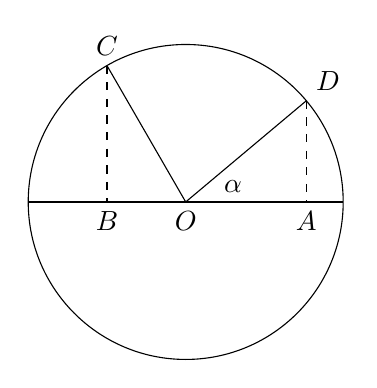
\begin{tikzpicture}[scale=2]
	\draw (0 , 0) circle (1);
	\draw (-1 , 0) -- (0 , 0) node[below]{$O$} -- (1 , 0);
	\draw [dashed](40:1)node[above right]{$D$} -- ({cos(40)} , 0)node[below]{$A$};
	\draw [dashed](120:1)node[above]{$C$} -- ({cos(120)} , 0)node[below]{$B$};
	\draw (0 , 0) -- (120:1);\draw (0 , 0) -- (40:1);
	\draw (0 . 3 , 0 . 1) node{$\alpha$};
\end{tikzpicture}


应用三角恒等式
\[
2 \cos 3 \alpha=8 \cos ^{3} \alpha-6 \cos \alpha
\]
而且令 $x=2 \cos \alpha$ ,  则有
\[
2 \cos 3 \alpha=x^{3}-3 x
\]
因为 $3 \alpha=120^{\circ} ,  \cos 3 \alpha=-1 / 2 ;$ 所以上面的方程式可以写作
\[
x^{3}-3 x+1=0
\]
这正是我们以前讨论过的方程式 . 

现在假说所给的只有单位长 , 我们可以作出一个半径是单位 长的圆 , 而且可以作 $O B=1 / 2$ ,  于是 $\angle A O C=120^{\circ}$ 因为所给的只
有单位长 , 所以我们的数域当限定是有理数域 . \footnote{因为从 $1$ 单用四种有理运算 ,  我们可以作出一切有理数 ,  即有理数域 . }

所以要解这个方程式 , 必须将一个立方根加入于有理数域中\footnote{参看前面几页 . } . 然而一个立方根是不能用直尺与圆规作出的 . 这样 , 我们可以知道: 用直尺与圆规三等分任意角是不可能的 . 

以相似的方法 , 不难证明用直尺、圆规解决立方倍积问题也是不可能的 . 对于这个问题 , 方程式是
\[
x^{3}=2
\]
数域是有理数域 . 这方程式在这个数域中的群含有六个置换 . 读者当证明须加入一个平方根和一个立方根于有理数域中 , 方程式的群才会变成 $1$  . 又因一个立方根是不能用直尺、圆规作出的 , 所以我们这个立方倍积问题是不可能的 . 

仿此 , 我们可以应用群论去探讨正多边形作图的问题\footnote{参考 L . E . Dickson: Modern Algebraic Theories ,  Chapter XI . } . 

\section{伽罗瓦的鉴定为什么是对的}

现在我们要证明一个方程式若有一个可解群 , 这方程式就可用根式解\footnote{我们不征此处证明这定理的逆定理 . 关于此点 , 读者可参考 L .  E .  Dickson:
	Modern Algebraic Theories , p . 198 . } . 

每个人在他少年的时候也许都有过这个经验: 想应运方程式
的根与系数之类系去解方程式 . 例如在二次方程式
\[
x^{2}+b x+c=0
\]
的两个根 $x_{1} ,  x_{2}$ 中 , 我们知道有
\[
x_{1}+x_{2}=-b \quad (1)
\]
与
\[
x_{1} x_{2}=c \quad (2)
\]
的关系 . 那末 , 我们为什么不从这两个方程式中去解 $x_{1} ,  x_{2}$ 呢? 我 们很容易发见这条路是走不通的 , 因为如果从(1)中得出 $x_{1}$ 的值 . 而后代入(2)中 , 结果是
\[
x_{2}^{2}+b x_{2}+c=0 , 
\]
这正与原来的二次方程式丝毫也没分别 . 所以这个法子只令我们兜了一个圈子又回到原来的出发点去了 . 但是 , 如果我们能得到一对都是一次的方程式 , 那末 ,  $x_{1}$ 和 $x_{2}$ 就实实在在可以求得了\footnote{但须假定这对方程式的系数之行列式不等于零 . } . 

如果方程式的群是一个元数为质数的巡回正置换群 , 那末 , 这方程式的确可以照刚才所说的法子去解 . 这一点我们立刻就要说明 , 而且我们还要观察这个特殊情形与一般的有可解群的方程式有什么关系 . 

现在先就这特殊情形来考究 , 设方程式
\[
f(x)=0
\]
有 $n$ 个相异的根 , 而且在那个由方程式的系数及 $1$ 之 $n$ 个 $n$ 次根决定的数域中\footnote{凡数域都含有一切有理数 , 因为我们若取数域中的任意一数来除他自己 ,  即得$1$  . 从 $1$ 应用有理运算 , 可得一切有理数 . 所以在任何数域中都含有一切有理数 . } , 此方程式的群是一个元数为质数的 巡回正置换群 . 

在此我们先要问什么叫做 1 之 $n$ 个 $n$ 次根 . 我们都知道 1 有 三个立方根\footnote{因为 $x^{3}=1 $ 可以写作$x^{3}-1=0$或$(x-1)\left(x^{2}+x+1\right)=0 , $由此即易得这三个根 . }
\[
1 , -\frac{1}{2}+\frac{1}{2} \sqrt{-3} , -\frac{1}{2}-\frac{1}{2} \sqrt{-3} . 
\]
(通常都记作 $1 ,  \omega ,  \omega^{2}$ )仿此 , 在一般的情形 ,  $1$ 有 $n$ 个 $n$ 次根 , 这 $n$个 $n$ 次根我们记作
\[
1 ,  \rho ,  \rho^{2} ,  \cdots ,  \rho^{n-1}
\]
1 的三个立方根只包含有理数和有理数的 根数 , 同样 $1$ 的 $n$ 个次根也只包含有理数和有理数的根数 . 所以这种数加入数域中去 时并不影响到“方程式是能用根式解”的这句命辞 . 

因为我们假定这方程式的群是一个元数为质数的巡回正置换群 , 群中的元素都是置换
\[(123……n)\]
的乘幂 , 这个置换的$n$次乘幂就是不动置换\footnote{见前面几页 . } . 

现在我们要应用一组一次方程式
\[
x_{1}+\rho^{k} x_{2}+\rho^{2 k} x_{3}+\cdots+\rho^{(n-1) k} x_{n}=\gamma_{k} , \quad (3)
\]
此处 $k$ 的值得为 $0$ 与 $n-1$ 间之任何整数 , 所以这是将 $n$ 个方程式
写作一个的简便写法 . 例如当 $k=0$ 时 , $(3)$就成为
\[
x_{1}+x_{2}+x_{3}+\cdots \cdots+x_{n}=\gamma_{0}
\]
当 $k=1$ 时 ,  $(3)$成为
\[
x_{1}+\rho x_{2}+\rho^{2} x_{3}+\cdots \cdots+\rho^{n-1} x_{n}=\gamma_{1}
\]
等等 . 

因为一个方程式的最高次项系数若是 $1$ , 则诸根之和等于方程式中第二项的系数的负值 , 所以 $\gamma_{0}$ 之值可以直接从方程式的系数中求得 . 现在要将置换
\[
(123 \cdots n)
\]
施行于$(3)$的左端 ,  $(3)$式左端就成为
\[
x_{2}+\rho^{k} x_{3}+\rho^{2 k} x_{4}+ \cdots+\rho^{(n-1) k} x_{1}
\]
但是若将$(3)$式左端用 $\rho^{-k}$ 一乘 , 也可得出同样的结果 , 这是因为
$\rho^{n}=1$ 的缘故 . 所以置换
\[
(123 \cdots n)
\]
将 $\gamma_{k}$ 之值变为 $\rho^{-k} \gamma_{k}$ .  又因 $\rho^{n}=1$ ,  故 $\left(\gamma_{k}\right)^{n}=\left(\rho^{-k} \gamma_{k}\right)^{n}$ ,  所以置换
\[
(123 \cdots \cdots n)
\]
不变更 $\gamma_{k}^{n}$ 的值 . 同样 , 群中其他的置换也不变 $\gamma_{k}^{n}$ 之值\footnote{因为这群是巡回群 , 群中的置换都是$(123\cdots n)$的乘幂 , 所以将群中某一置换施行于 $\gamma_{k}^{n}$ 实在就相当于将 $(123 \cdots n)$ 重复施行若干次于 $\gamma_{x_{\circ}}^{n}$ 但将 $(123 \ldots n)$施行一次于$\gamma_{x}^{n}$ 既不改变 $\gamma_{x}^{n}$ 的值 , 重复施行若干次当然也不变更 $\gamma_{x}^{n}$ 的值} . 

如此 , 群中一切置换既然都不变更 $\gamma_{k}^{n}$ 之值 ,  $\gamma_{k}^{n}$ 之值必在那数域中\footnote{参看前面几页 . } . 因此 ,  $\gamma_{k}$ 是数域中某一个数的 $n$ 次根 . 这就是说: 所有 $\gamma$ 的值都可由根式得到(对于那数域而言!) . 而由 $(3)$ 中可以将$x$ 用 $\rho$ 与 $\gamma$ 表出 , 于是这组方程式$(3)$是可以用根式解的 . 但是这些 $x$ 就是方程式 $f(x)=0$ 的根 . 所以我们已经证明: 如果方程式在一个数域中的群是元数为质数的巡回正置换群 , 则此方程式必可用根式解 . 

举例来说: 方程式
\[
x^{3}-3 x+1=0
\]
在有理数域中的群是 $1 ,  (123) ,  (132)$\footnote{参看前面几页 . }; 这是一个元数为质数的 巡回正置换群 , 所以我们可以从
\[
\begin{array}{c}
	x_{1}+x_{2}+x_{3}=0 \\
	x_{1}+\omega x_{2}+\omega^{2} x_{3}=\gamma_{1} \\
	x_{1}+\omega^{2} x_{2}+\omega x_{3}=\gamma_{2}
\end{array}
\]
这三个一次方程式中解它 . 此处 $\omega$ 表示 $1$ 的一个虚立方根 , $\gamma_{1}$ 与$\gamma_{2}$ 可以由数域中的数的根数而得 . 换句话说 , 如果把这种根数加入到数域中去 , 则 $x$ 都存在于扩大的数域中 . 

但是 , 假使方程式的群不是一个元数为质数的巡回正置换群 , 那又怎么样呢?

方程式的群是一个可解群时 , 他的解法在第 35 页中已说了一 个梗概 . 在那里我们已经知道: 假使组合因数都是质数 , 虽则方程式的群不是一个元数为质数的巡回正置换群 , 这方程式还是能用根式解的 . 因为这时候每个辅助方程式在那个用前几个辅助方程式的根扩大成的数域中的群是一个元数为质数的巡回正置换群 . 

如此 , 每个辅助方程式既有一个元数为质数的巡回正置换群 ,  根据以前所说的 , 这些辅助方程式都能用根式解 . 所以这些加入原来的数域去的辅助方程式的根 , 都只不过是原来的数域中的数的根数而已 . 这样看来 , 只要方程式的群是可解群 , 这方程式就是能用根式解的 . 

在一般的情形 , 我们常可以取
\[
y^{2}=\left(x_{1}-x_{2}\right)^{2}\left(x_{1}-x_{3}\right)^{2}  \cdots \left(x_{n-1}-x_{n}\right)^{2}
\]
作第一个辅助方程式 , 此式右端是所有每两个根之差的平方之积 . 假若方程式的第一项系数是 $1$ 的话 , 那末 , 上式的右端正是方程式的\emph{判别式}(Discriminant) . 例如二次方程式
\[
x^{2}+b x+c=0
\]
的两个根 $x_{1} ,  x_{2}$ 之差之平方是
\[
\left(x_{1}-x_{2}\right)^{2}=\left(x_{1}+x_{2}\right)^{2}-4 x_{1} x_{2}=b^{2}-4 c
\]
这恰是方程式的判别式 . 同样 , 高次方程式的判别式也可从系数求得 . 现在第一个辅助方程式的两个根就是这判别式的两个平方根 , 将这两个平方根加入数域中 , 方程式在这新的数域 $F_{1}$ 中的群是 $H$ .  我们再照同样方法用其余的辅助方程式进行下去 . 

设若所要解的方程式是一个一般的三次方程式 , 将第一个辅助方程式的根加入原来的数域之盾 , 方程式的群变为 $H_{\circ}$ 在这情形 ,  $H$ 是一个元数为质数的巡回正置换群 . 所以我们可以利用
\[
\begin{array}{r}
	x_{1}+x_{2}+x_{3}=-b \\
	x_{1}+\omega x_{2}+\omega^{2} x_{3}=\gamma_{1} \\
	x_{1}+\omega^{2} x_{2}+\omega x_{3}=\gamma_{2}
\end{array}
\]
这三个一次方程式来解原来的三次方程式 . 此中的 $\gamma_{1} ,  \gamma_{2}$ 可由数域(这数域是由三次方程式的系数以及第一个辅助方程式的根而决定的)中的数之根数求得\footnote{参考 L . E . Dickson:Modem Algebraic Theories , p  . 136 . 但此处的$\gamma_{1} ,  \gamma_{2}$该书中记作$\fi \psi $} . 换句话说 , 假使把 $\gamma_{1} ,  \gamma_{2}$ 的值也加入数域中 , 则方程式的群变为 $1$  . 这也就是说 ,  $x_{1} ,  x_{2} ,  x_{3}$ 存在于这个最后经 $\gamma_{1} ,  \gamma_{2}$ 之加入而扩大成的数域中 . 

如此我们已经证明: 方程式在一个由其系数与 $1$ 之 $n$ 个 $n$ 次根而决定的数域中的群若是一个可解群 , 则此方程式是可以用根式解的 . 

当然 , 如果方程式在一个含有其系数的数域中的群是可解群 ,  则对于这数域而言 , 此方程式是可以用根式解的 .  本书所说的已够使读者知道一个大概 , 我们希望读者继续去 研究这门引人入胜的数学 . 要知道用群论解方程式并不是这个令 人惊叹的群的概念的惟一应用 . 

应用群论于几何学\footnote{参考 Veblen and Young:Projective Geometry . } , 使几何学起了一个大的改革 . 还有在 相对论中 , 群论也极重要 . 培尔(E .  $\mathrm{T}  .  \mathrm{Bell}$ )说过\footnote{参看 E . T . Belk:The Queen of the Sciences 及 C . J . Keyser: Mathematical Philosophy 一书中论群之概念一章 . } “无论在什么地方 ,  只要能应用群论 , 从一切纷乱混淆中立刻结晶出简洁余和谐 .  群的概念是近世纪科学思想的出色的新工具之一 . ”

\section{要义}
1 . 数学并不像普通一般人所相信的 , 仅是一组呆板的定义和 法则 . 在把人们的心从他的偏见和旧的定义中解放出来以后 , 现 代的数学已开辟了一块非常膏腴的园地(参阅第95-98页) . 

2 . 不过这种解放绝对不是纷乱无主的 , 在推广了定义、选定 了公理和确定了数域以后 , 我们就要遵从这些限制 , 只要我们在这 一个系统里研究的话 , 对于他们就要表示忠诚(参阅第89—91页) . 

3 . 然则 , 在起初的 时候我们将如何选择那 些公理和定义以及数域 呢 , 那是要看目的如何 而定的 . 如伽罗瓦的目 的是要用既定的方法来 解方程式(参阅第88— 91 页) . 

4 . 有了目的 , 有了 和这目的契合的公理 ,  那末 , 方法又怎样呢? 这方法就是要用一个以 一些变化作元素的群之 元素来变化那些我们所 研究的东西 , 并且找出 对于这些变化不会更易的东西 , 这些在我们的 系统中是不会变更的 . 

5 . 从现代数学中可以得到的另一个训示是:一个很小的原因 可以引起惊人的结果 . 这正是:“星星之火 , 可以燎原” . 一个问题 可以是可能的或不可能的 , 只要在条件上有点轻微的变更(参阅第 90-91页) . 这个拿几何学最好做比喻:只在一条公理上有一点 细微的变化 , 把其余的公理照旧 , 就把欧几里得几何学变成非欧几 里得几何学了\footnote{参看本书作者所著之 Non-Euclidian Geometry or Three Moons in Mathesis 一书 . } . 

